%!TEX root = ../main.tex
%=========================================================

\section{Introduction}

Ethereum is one of \er{or \textbf{the} largest?} the largest decentralized platform currently in operation. \er{see the official numbers, 27.000 nodes in total? Source?}
While is is widely known for supporting the blockchain of the same name (also known as the \emph{mainnet}), the Ethereum platform is also home to a number of additional decentralized applications.
This includes blockchains used for test purposes (testnets such as \emph{Ropsted} or \emph{Rinkeby}), divergent blockchains resulting from a past fork (\emph{Ethereum classic}), alternative cryptocurrencies (\emph{Pirl}, \emph{Musicoin}), content delivery networks (\emph{Swarm}), or messaging applications (\emph{Whisper}). \er{maybe give more/more diversified examples? IPFS? Others? Why isn't IPFS on the plot btw?}
In 2018, a study of the Ethereum ecosystem~\cite{kim2018measuring} indicated that the platform featured no less than 4,076 of them, and that this number will keep growing in the future. \er{this really reads as if the paper was written in 2018, don't we have more recent numbers? Ideally we would like to have them for several years and show the trend.}

\begin{figure}[t]
    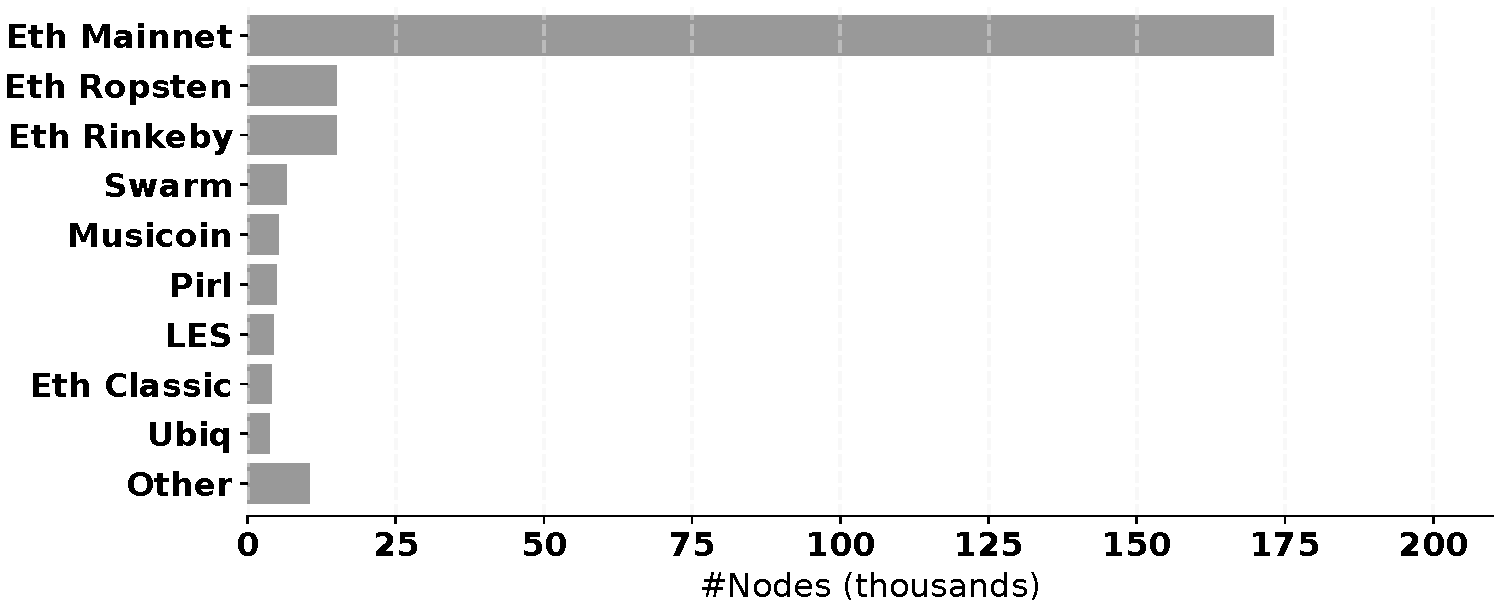
\includegraphics[width=1\linewidth]{img/ecosystem}
    \caption{Number of different nodes identities witnessed in Ethereum's main applications, over an observation period of one year \protect\er{was it one year exactly?} (numbers reported by Kim et al.~\cite{kim2018measuring}).
    \protect\er{maybe give the date when the snapshot was taken. Also, ``Other'' should be ``Others''. We can also consider using a split x axis in order to avoid the very small lines for everything else than the mainnet. The figure is also not giving a sense of the long tail with networks of a few hundreds/thousands of nodes (our focus)}
    \protect\er{present relative numbers rather than absolute ones}
    }
    \label{fig:ecosystem}
\end{figure}

Every node in the Ethereum platform participates to a \emph{global} peer-to-peer (P2P) network operating the Kademlia distributed hash table (DHT)~\cite{maymounkov2002kademlia}. \er{how many nodes in this global network?}
Bootstrapping membership to this general network is handled by a number of trusted \emph{bootstrap nodes} operated by the Ethereum foundation, who provide an initial list of contact peers to nodes entering the network.
Once joined, every node must connect to one or more sub-network(s) formed of peers participating to its application(s) of interest.
The size of these sub-networks can vary significantly.
\Cref{fig:ecosystem} depicts the size distribution of the platform main applications.
This distribution features a \emph{long tail}, with a vast majority of applications formed of a few thousand nodes or less, much less than the mainnet or the testnets. \er{would be useful to give more precise quantiles, e.g., 80\% have less than 1.000 nodes, 90\% less than 200 nodes, etc.}

In this paper, we focus on the \emph{service discovery} mechanism, by which a newly-joined node discovers a subset of peers already members of an application's sub-network.
This set of peers are then contacted in order to join the P2P overlay specific to that application, as illustrated by \Cref{fig:subnetwork}.

\begin{figure}[b!]
    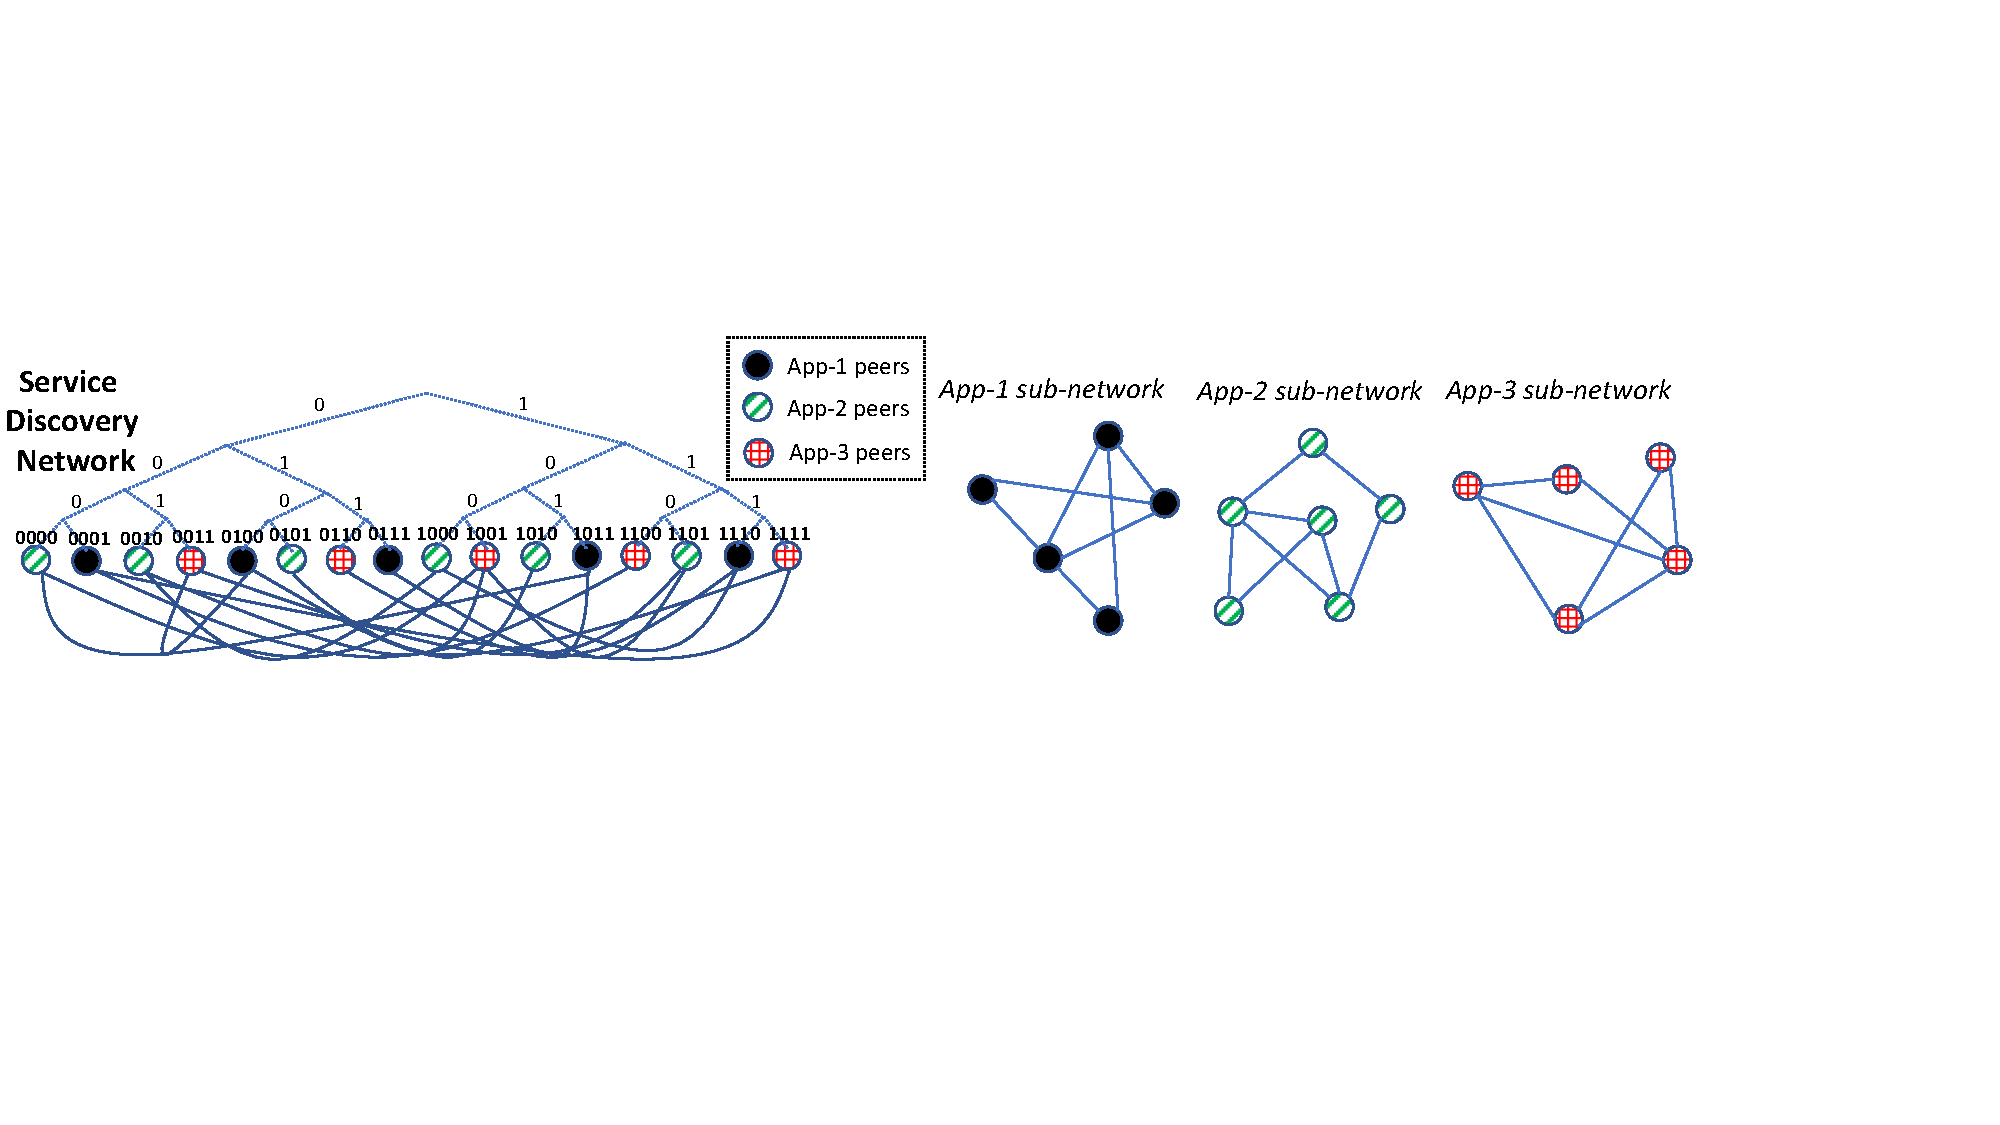
\includegraphics[width=1\linewidth]{img/subnetwork}
    \caption{Formation of application-specific sub-networks using a universal service discovery network.
    \protect\er{would be good to use different structures for the sub-networks, here they look quite similar}
    }
    \label{fig:subnetwork}
\end{figure}

Service discovery is a particularly sensitive mechanism in the Ethereum platform.
Its implementation must ensure, indeed, that malicious participants to this open network are unable to bias its execution in their favor or against a victim--and that, despite the ability of these adversaries to establish and operate multiple Sybil identities.
Of particular importance is the protection against \emph{eclipse} attacks, where an adversary would lure its victim(s) into a sub-network formed of only nodes under its control. %, i.e., by returning only such nodes to a service discovery request.
Similarly, an adversary could wish to run \emph{denial-of-service} attacks against a specific application, preventing other nodes from discovering peers from its associated sub-network.
On the other hand, the mechanism must remain efficient and scalable.
It is not desirable, in particular, that it relies on a set of \emph{centralized} registry nodes maintaining the membership of each and every application, both for scalability and governance reasons.
% \er{also the applications may want to hide themselves (but this clashes completely with our announcement approach)}

The current service discovery mechanism used in the Ethereum platform is part of discv4, a set of protocols using the global Kademlia DHT.
It employs a simple but robust \emph{random walk} approach.
A node willing to join an application's sub network simply contacts in sequence a series of nodes collected from the DHT, asking for application membership until it has collected enough peers. % to join the sub-network.
This approach offers good resilience to malicious behaviors
% , and in particular against denial-of-service attacks, 
but it suffers from very poor scalability and performance, in particular for small sub-networks.
While using the Kademlia DHT as a key/value store to maintain membership information at a specific node or replica group would allow deterministic lookup of this information, regardless of the application's popularity, this solution would suffer from very poor robustness to attacks and would lead to hotspots and overload for nodes in charge of popular services.

\smallskip
\noindent
\textbf{Contributions.}
%
We detail in this paper \sysname, a novel service discovery mechanism for large-scale, decentralized platforms and its application to the Ethereum platform.
\sysname has been already integrated into the upcoming version of Ethereum, as part of the replacement of discv4 mechanisms ... \er{provide details here already. Why don't we call it discv5 anymore?}

Outline for the rest of the section, to be discussed
\begin{itemize}
  \item \sysname does not keep membership information only at the nodes participating to the sub-networks, as in discv4, but allows these nodes to register their association with specific applications; the registrations are stored in a specific part of the global DHT overlay. However, in contrast with \emph{classical} DHT routing, these registrations are more widely spread to reduce the ability of attackers to delete or tamper with membership information
  \item \sysname operates a bias between well-represented services and small ones such that the probability of finding peers for low-popularity applications remains sufficiently high (to be rephrased better) \er{side question: how do we prevent small applications for being easier to attack with eclipse attacks than large ones? Diversity is also a tool in the hand of the attacker allowing it to register more Sybils, isn't it?}
  \item \sysname limits the amount of storage and state each node maintains and implements a novel admission protocol that ...
\end{itemize}

% To be continued:
% \begin{itemize}
%   \item why using the DHT directly is also not acceptable as it is efficient and scalable but easily attacked (we need references for this)
%   \item our contributions
%   \item summary of evaluation and integration in Ethereum
% \end{itemize}
